\documentclass[12pt,reqno,final,pdftex]{amsart}\usepackage[]{graphicx}\usepackage[]{color}
%% maxwidth is the original width if it is less than linewidth
%% otherwise use linewidth (to make sure the graphics do not exceed the margin)
\makeatletter
\def\maxwidth{ %
  \ifdim\Gin@nat@width>\linewidth
    \linewidth
  \else
    \Gin@nat@width
  \fi
}
\makeatother

\definecolor{fgcolor}{rgb}{0.345, 0.345, 0.345}
\newcommand{\hlnum}[1]{\textcolor[rgb]{0.686,0.059,0.569}{#1}}%
\newcommand{\hlstr}[1]{\textcolor[rgb]{0.192,0.494,0.8}{#1}}%
\newcommand{\hlcom}[1]{\textcolor[rgb]{0.678,0.584,0.686}{\textit{#1}}}%
\newcommand{\hlopt}[1]{\textcolor[rgb]{0,0,0}{#1}}%
\newcommand{\hlstd}[1]{\textcolor[rgb]{0.345,0.345,0.345}{#1}}%
\newcommand{\hlkwa}[1]{\textcolor[rgb]{0.161,0.373,0.58}{\textbf{#1}}}%
\newcommand{\hlkwb}[1]{\textcolor[rgb]{0.69,0.353,0.396}{#1}}%
\newcommand{\hlkwc}[1]{\textcolor[rgb]{0.333,0.667,0.333}{#1}}%
\newcommand{\hlkwd}[1]{\textcolor[rgb]{0.737,0.353,0.396}{\textbf{#1}}}%
\let\hlipl\hlkwb

\usepackage{framed}
\makeatletter
\newenvironment{kframe}{%
 \def\at@end@of@kframe{}%
 \ifinner\ifhmode%
  \def\at@end@of@kframe{\end{minipage}}%
  \begin{minipage}{\columnwidth}%
 \fi\fi%
 \def\FrameCommand##1{\hskip\@totalleftmargin \hskip-\fboxsep
 \colorbox{shadecolor}{##1}\hskip-\fboxsep
     % There is no \\@totalrightmargin, so:
     \hskip-\linewidth \hskip-\@totalleftmargin \hskip\columnwidth}%
 \MakeFramed {\advance\hsize-\width
   \@totalleftmargin\z@ \linewidth\hsize
   \@setminipage}}%
 {\par\unskip\endMakeFramed%
 \at@end@of@kframe}
\makeatother

\definecolor{shadecolor}{rgb}{.97, .97, .97}
\definecolor{messagecolor}{rgb}{0, 0, 0}
\definecolor{warningcolor}{rgb}{1, 0, 1}
\definecolor{errorcolor}{rgb}{1, 0, 0}
\newenvironment{knitrout}{}{} % an empty environment to be redefined in TeX

\usepackage{alltt}
%% DO NOT DELETE OR CHANGE THE FOLLOWING TWO LINES!
%% $Revision$
%% $Date$
\usepackage[round,sort,elide]{natbib}
\usepackage{graphicx}
\usepackage{times}
\usepackage{rotating}
\usepackage{subfig}
\usepackage{comment}
\usepackage{color}
\newcommand{\aak}[1]{\textcolor{cyan}{#1}}
\newcommand{\mab}[1]{\textcolor{red}{#1}}
\newcommand{\cec}[1]{\textcolor{blue}{#1}}

\setlength{\textwidth}{6.25in}
\setlength{\textheight}{8.75in}
\setlength{\evensidemargin}{0in}
\setlength{\oddsidemargin}{0in}
\setlength{\topmargin}{-.35in}
\setlength{\parskip}{.1in}
\setlength{\parindent}{0.3in}

%% cleveref must be last loaded package
\usepackage[sort&compress]{cleveref}
\newcommand{\crefrangeconjunction}{--}
\crefname{figure}{Fig.}{Figs.}
\Crefname{figure}{Fig.}{Figs.}
\crefname{table}{Table}{Tables}
\Crefname{table}{Tab.}{Tables}
\crefname{equation}{Eq.}{Eqs.}
\Crefname{equation}{Eq.}{Eqs.}
\crefname{appendix}{Appendix}{Appendices}
\Crefname{appendix}{Appendix}{Appendices}
\creflabelformat{equation}{#2#1#3}

\theoremstyle{plain}
\newtheorem{thm}{Theorem}
\newtheorem{corol}[thm]{Corollary}
\newtheorem{prop}[thm]{Proposition}
\newtheorem{lemma}[thm]{Lemma}
\newtheorem{defn}[thm]{Definition}
\newtheorem{hyp}[thm]{Hypothesis}
\newtheorem{example}[thm]{Example}
\newtheorem{conj}[thm]{Conjecture}
\newtheorem{algorithm}[thm]{Algorithm}
\newtheorem{remark}{Remark}
\renewcommand\thethm{\arabic{thm}}
\renewcommand{\theremark}{}

\numberwithin{equation}{part}
\renewcommand\theequation{\arabic{equation}}
\renewcommand\thesection{\arabic{section}}
\renewcommand\thesubsection{\thesection.\arabic{subsection}}
\renewcommand\thefigure{\arabic{figure}}
\renewcommand\thetable{\arabic{table}}
\renewcommand\thefootnote{\arabic{footnote}}

\newcommand\scinot[2]{$#1 \times 10^{#2}$}
\newcommand{\code}[1]{\texttt{#1}}
\newcommand{\pkg}[1]{\textsf{#1}}
\newcommand{\dlta}[1]{{\Delta}{#1}}
\newcommand{\Prob}[1]{\mathbb{P}\left[#1\right]}
\newcommand{\Expect}[1]{\mathbb{E}\left[#1\right]}
\newcommand{\Var}[1]{\mathrm{Var}\left[#1\right]}
\newcommand{\dd}[1]{\mathrm{d}{#1}}
\newcommand{\citetpos}[1]{\citeauthor{#1}'s \citeyearpar{#1}}
\IfFileExists{upquote.sty}{\usepackage{upquote}}{}
\begin{document}



\subsection*{Preliminaries}
The data that we are trying to fit with the full DEB model with parasitism is of the body size and parasite load of individual \emph{Daphnia}.
Before attempting to fit all of this data, it is worth attempting to fit only the growth data.
This is because, if we cannot fit the growth data, we will not be able to fit both the growth and parasite load data.
Moreover, fitting only the growth data is more straightforward, as we already have a good model for growth.
My assumption (and the assumption of most people), is that \emph{Pasteuria} modifies the growth of individual \emph{Daphnia} by increasing the fraction of mobilized energy that is allocated towards growth ($\kappa$).
In so doing, the parasite causes both gigantism and castration.
However, it is worth asking whether the parasite also modifies other aspects of the energy budget, especially in light of the fact that infection causes a reduction in host foraging.
This reduction in resource ingestion could compromise the ability to induce gigantism.
To address this question, I will fit the following model to the growth data of infected animals:
\begin{align}
\frac{dF}{dt} &= -I_{max} \frac{F}{F_h+F} L^g, \\
\frac{dE}{dt} &= \rho \epsilon V I_{max} \frac{F}{F_h+F} L^g - \frac{E (v/L + k_m)}{1+\kappa E/W}, \\
\frac{dW}{dt} &= \kappa \frac{E (v/L + k_m)}{1+\kappa E/W} - k_m W.
\end{align}

I will assume that the energy budget parameters (the assimilation efficiency, $\rho$; the energy conductance, $v$; and the somatic maintenance rate, $k_m$) have the same value as in uninfected animals.
I will assume the the ingestion parameters (ingestion rate, $I_{max}$ and shape parameter $g$) take on the best-fitting values when this feeding model was fit to the ingestion data.
The half-saturation constant, $F_h$, proved impossible to estimate then, but based on Fig. 2 in the document ``Notes\_feeding\_model.pdf'', $g$ is nearly constant across a range of fixed $F_h$ values, whereas $I_{max}$ increases linearly with $F_h$.
I will assume $F_h=10000$, which implies that $g=0.156$ and $I_{max}=14250$.
The size of the experimental container $V$ and the carbon content of an algae cell $\epsilon$ are both fixed at their known values.
That leaves only the growth allocation $\kappa$ to be estimated.

The maximum likelihood estimate of $\kappa$, according to the data, is $\kappa=1$, as expected.
However, even with $\kappa=1$, the fit to the data is very poor (Fig. \ref{fig:inf-length}): the maximum possible size of the animals is far less than is actually observed in the data.
\textbf{This suggests that the parasite must be adjusting other aspects of the energy budget in order to induce gigantism, especially in the face of infection-induced foraging reduction.}
There are two possibilities: the parasite either reduces somatic maintenance rates or increases assimilation efficiency (modifying the energy conductance has no effect on the fit).

As an aside, this also explains past difficulties with fitting the parasite data: the model can't fit the observed growth \emph{before} adding a parasitic drain on reserves or biomass; with that additional drain on energy, there is no way to remotely fit the growth data.
In past fitting attempts, it was clear that the fitting algorithm was exploring parameter space where the impact of the parasite on the host energy budget was minimal, while simultaneously inflating the variance in parasite load measurement error.


\begin{knitrout}\scriptsize
\definecolor{shadecolor}{rgb}{0.969, 0.969, 0.969}\color{fgcolor}\begin{figure}


\includegraphics[width=\linewidth]{figure/inf-length-1} \hfill{}

\caption[The best-fitting growth model for infected animals when most of the parameters are held fixed at their uninfected values except for the feeding parameters (infected animals eat less) and the growth allocation $\kappa$]{The best-fitting growth model for infected animals when most of the parameters are held fixed at their uninfected values except for the feeding parameters (infected animals eat less) and the growth allocation $\kappa$. Even with $\kappa$ maximized, the model fits the data poorly - the animals are unable to grow as large as is observed in the actual data.}\label{fig:inf-length}
\end{figure}


\end{knitrout}

We can fit the model to the growth data to determine how much infection is adjusting these values.
If we allow the assimilation efficiency $\rho$ to vary, the model fit improves considerably (Fig. \ref{fig:inf-length-2}).
Allowing somatic maintenance rate to vary improves the fit even more.
In particular, if I only want to let infection adjust one parameter, the one that is best supported is the somatic maintenance rate, which is \emph{dramatically} reduced by infection (from an uninfected baseline of 0.073 to 0.0013).
If you let both parameters be flexible, then the best supported model is one where the parasite reduces assimilation effiency slightly while greatly reducing somatic maintenance rate.
\textbf{If we take this result seriously, it suggests that the metabolic rates of infected animals may be much lower than their uninfected counterparts.}

\begin{knitrout}\scriptsize
\definecolor{shadecolor}{rgb}{0.969, 0.969, 0.969}\color{fgcolor}\begin{figure}


\includegraphics[width=\linewidth]{figure/inf-length-2-1} \hfill{}

\caption[Best-fitting growth trajectories when parasites are able to adjust growth allocation and either assimilation efficiency, somatic maintenance rate, or both]{Best-fitting growth trajectories when parasites are able to adjust growth allocation and either assimilation efficiency, somatic maintenance rate, or both.}\label{fig:inf-length-2}
\end{figure}


\end{knitrout}

\subsection*{Models of parasite growth and development}

There are many different possibilities for the model of parasite replication, but I want to consider three basic variants that differ in terms of where the parasite gets its energy.
The first assumes that parasites use reserves as a resource, as in Hall et al. 2009.
The second assumes that parasites use soma as a resource.
Within each of these different energetic architectures, there are multiple possible ways to model parasite replication and development, so I will consider several variants for each.

\subsection*{Models of exploitation of reserves}
Here I will assume that \emph{Pasteuria} exploits reserves, so there will be an additional negative term in the $dE/dt$ equation which is the parasite's ``functional response'', $a_P P$.
The parasite's equation will take one of five forms:
\begin{align}
(1) \frac{dP}{dt} &= \epsilon_P a_P E P, \\
(2) \frac{dP}{dt} &= \epsilon_P a_P E P - m P, \\
(3) \frac{dP}{dt} &= \epsilon_P a_P E P \left(1 - \frac{P}{k_P W}\right).
\end{align}
The third equation assumes that the parasite's growth rate is
logistic, with a carrying capacity that is determined by the
\emph{size} of the host.
This makes sense, especially for \emph{Pasteuria}, as the parasite
essentially completely fills the hemolymph near the end of infection,
and it is thought that the benefit of gigantism to the parasite might
simply be that it increases the total volume that can be filled with
parasite spores.

I also consider structured-population versions of these equations,
where the parasite can be divided into replicating and non-replicating
stages ($P_i$ and $P_m$).
I assume that the replicating stage exploits resources eventually
matures into a non-replicating stage.
This approximates our best understanding of the biology of
\emph{Pasteuria}, which has several stages; the final stage is what is
actually counted, and as it is an endospore, it is likely fairly inert in
the host.
Rather than assuming an exponentially distributed waiting time in the
replicating stage, I assume a fixed delay $\tau$, that is the duration
of the replicating stage.
The fourth model is then
\begin{align}
(4a) \frac{dP_i(t)}{dt} &= \epsilon_P a_P E(t) P_i(t) - \epsilon_P a_P
                          E(t-\tau) P_i(t-\tau), \\
(4b) \frac{dP_m(t)}{dt} &= \epsilon_P a_P E(t-\tau) P_i(t-\tau).
\end{align}
The fifth model is slightly more complicated, because we have to take
into consideration the mortality of the replicating stage.
Since the mortality rate is $m$, the probability that an replicating
stage parasite survives $\tau$ time units and matures is $e^{-m
  \tau}$, so the model of parasite growth and development is:
\begin{align}
(5a) \frac{dP_i(t)}{dt} &= \epsilon_P a_P E(t) P_i(t) - e^{-m \tau}\epsilon_P a_P
                          E(t-\tau) P_i(t-\tau), \\
(5b) \frac{dP_m(t)}{dt} &= e^{-m \tau} \epsilon_P a_P E(t-\tau) P_i(t-\tau).
\end{align}
The sixth model again assumes logistic growth with a carrying capacity
determined by size.
I assume that both replicating and non-replicating stages contribute
to the carrying capacity.
\begin{align}
(6a) \frac{dP_i(t)}{dt} &= \epsilon_P a_P E(t) P_i(t) \left(1 -
                          \frac{P_i(t)+P_m(t)}{k_P W(t)}\right) - \epsilon_P a_P E(t-\tau) P_i(t-\tau) \left(1 -
                          \frac{P_i(t-\tau)+P_m(t-\tau)}{k_P
                          W(t-\tau)}\right) \\
(6b) \frac{dP_m(t)}{dt} &= \epsilon_P a_P E(t-\tau) P_i(t-\tau) \left(1 -
                          \frac{P_i(t-\tau)+P_m(t-\tau)}{k_P W(t-\tau)}\right).
\end{align}

\subsection*{Models of exploitation of soma}
Here I will assume that \emph{Pasteuria} exploits somatic mass, so there will be a negative term in the $\frac{dW}{dt}$ term.
Otherwise, the size possible forms for the growth equation parallel those in the model of reserve exploitation:
\begin{align}
(7) \frac{dP}{dt} &= \epsilon_P a_P W P, \\
(8) \frac{dP}{dt} &= \epsilon_P a_P W P - m P, \\
(9) \frac{dP}{dt} &= \epsilon_P a_P W P \left(1 - \frac{P}{k_P W}\right).
(10a) \frac{dP_i(t)}{dt} &= \epsilon_P a_P W(t) P_i(t) - \epsilon_P a_P
                          W(t-\tau) P_i(t-\tau), \\
(10b) \frac{dP_m(t)}{dt} &= \epsilon_P a_P W(t-\tau) P_i(t-\tau).
(11a) \frac{dP_i(t)}{dt} &= \epsilon_P a_P W(t) P_i(t) - e^{-m \tau}\epsilon_P a_P
                          W(t-\tau) P_i(t-\tau), \\
(11b) \frac{dP_m(t)}{dt} &= e^{-m \tau} \epsilon_P a_P W(t-\tau) P_i(t-\tau).
(12a) \frac{dP_i(t)}{dt} &= \epsilon_P a_P W(t) P_i(t) \left(1 -
                          \frac{P_i(t)+P_m(t)}{k_P W(t)}\right) - \epsilon_P a_P W(t-\tau) P_i(t-\tau) \left(1 -
                          \frac{P_i(t-\tau)+P_m(t-\tau)}{k_P
                          W(t-\tau)}\right) \\
(12b) \frac{dP_m(t)}{dt} &= \epsilon_P a_P W(t-\tau) P_i(t-\tau) \left(1 -
                          \frac{P_i(t-\tau)+P_m(t-\tau)}{k_P W(t-\tau)}\right).
\end{align}

\begin{comment}
\subsection*{Models of exploitation of growth allocation}
These models are slightly more complicated, and fall into two classes.
In the first, \emph{Pasteuria} diverts a constant fraction, $\phi$ of growth allocation towards itself.
$\phi$ is assumed to be constant and independent of parasite population size.
This reduces growth allocation from $\kappa p_C$ to $(1-\phi) \kappa p_C$.
We consider three possible parasite growth functions:
\begin{align}
(11) \frac{dP}{dt} &= \epsilon_P \phi \kappa p_C, \\
(12) \frac{dP}{dt} &= \epsilon_P \phi \kappa p_C - m P, \\
(13) \frac{dP}{dt} &= \epsilon_P \phi \kappa p_C \left(1 - \frac{P}{k_P W}\right).
\end{align}

The second class of models assumes that the fraction of growth allocation that is diverted towards the parasite is dependent on the parasite abundance.
Specifically, we assume that the fraction diverted is $\phi \frac{P}{h_P + P}$, so that the fraction diverted asymptotically approaches $\phi$ and $P$ approaches infinity.
We consider the same three model variants as before:
\begin{align}
(14) \frac{dP}{dt} &= \epsilon_P \phi \frac{P}{h_P + P} \kappa p_C, \\
(15) \frac{dP}{dt} &= \epsilon_P \phi \frac{P}{h_P + P} \kappa p_C - m P, \\
(16) \frac{dP}{dt} &= \epsilon_P \phi \frac{P}{h_P + P} \kappa p_C \left(1 - \frac{P}{k_P W}\right).
\end{align}

\subsection*{Fitting parasite growth data alone}
Given the utility of fitting the body size data alone, before I attempt to fit both the body size and parasite spore data simultaneously, it makes sense to see if there is anything to be learned from fitting the spore data alone.
In this case, I will assume that $E$ or $W$ is specified, and fit the competing parasite models to the spore data alone.
This will give me some information about how difficult the spore data is going to be to fit on its own, as well as providing some ballpark estimates for the different parameters.

If I look at the outputs of $E$ and $W$ from the best-fitting model of infected growth (see Fig. \ref{fig:inf-length-2}), I can get reasonable estimates for $E$ and $W$.
In particular, $E$ is bounded between about 3e-5 and 4e-5, whereas $W$ obviously changes over time.
To fit parasite data only, I either assumed a constant reserve $E=3\times10^{-5}$ or a growth somatic mass $W$, where mass was determined at each time point by a cubic regression of observed growth on age.
I did not carry out a full fitting study, as I only ran a single optimization from a single set of starting points.
The purpose was just to see whether some of the model fits would immediately give confidence that the algorithm had some chance of actually fitting the data.
The results (Fig. \ref{fig:parasite-only}) are fairly informative in that regard.
The Type I functional response is, essentially, a non-starter. The fits were horrible for both resource models.

\begin{knitrout}\scriptsize
\definecolor{shadecolor}{rgb}{0.969, 0.969, 0.969}\color{fgcolor}\begin{figure}

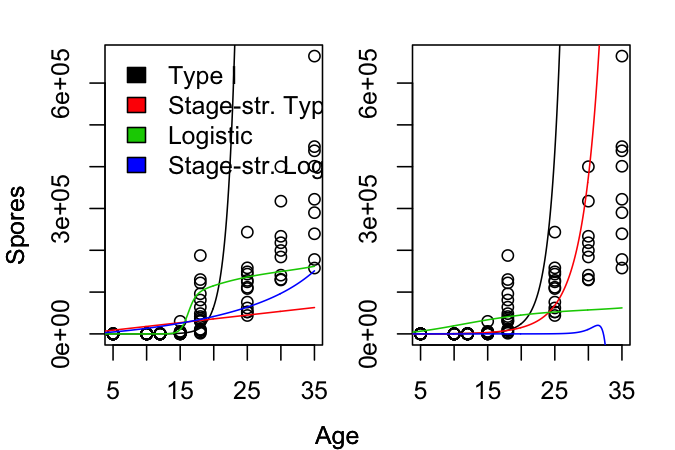
\includegraphics[width=\linewidth]{figure/parasite-only-1} \hfill{}

\caption[Fits of the parasite growth trajectory only, for 8 different models]{Fits of the parasite growth trajectory only, for 8 different models. The left-hand panel shows the best fits of models where the parasite exploits a constant reserve $E$; the right-hand panel shows the best fits of models where the parasite exploits somatic tissue $W$ (where the amount of somatic mass was set by the mean of a cubic regression on the actual observed parasite growth. For each parasite resource, we fit four models: a model with an unstructured parasite population with a Type I functional response, a model with an unstructured parasite population with resource-dependent and host size-dependent logistic growth (growth rate is determined by resources, carrying capacity is determined by host size), and structured population models of the same (immature and mature spores, where mature spores contribute to carrying capacity but do not reproduce).}\label{fig:parasite-only}
\end{figure}


\end{knitrout}

\end{comment}


\subsection*{Details of the fitting procedure}
In addition to estimating the parameters of the parasite growth equation (between two and four parameters), we also estimated the somatic maintenance rate of infected animals $k_m$ (based on our findings above), and a measurement error parameter.
The initial abundance of parasites is not a known quantity, as the hosts were exposed to a constant dose of parasite for a known duration, but a single spore can initiate infection in this system.
However, initial value parameters are notoriously difficult to
estimate, and can be difficult to constrain.
Thus I chose to assume an initial abundance of 100 replicating
parasites for each model.

Since the parasite population is growing, assuming normally distributed observation error with constant variance is potentially problematic.
Instead, we assumed that observation error was negative binomially distributed, with mean, $\mu$, given by the model, and the dispersion parameter, $s$, being estimated.
The variance of the negative binomial distribution is $\mu + \mu^2/s$, so that variance increases with the mean, a feature observed in the spore count data.

We also had to make assumptions about other physiological parameters.
We held all of the DEB parameters at the values estimated from the uninfected animals' growth and reproduction data except for the somatic maintenance rate and the allocation to growth, $\kappa$.
Because \emph{Pasteuria} is a castrating parasite, it is clear that $\kappa$ eventually becomes equal to one, but as none of the \emph{Daphnia} ever reproduced, it is very difficult to estimate \emph{when} $\kappa$ changes from its uninfected value to one.
For simplicity, therefore, we simply assumed that $\kappa = 1$ from birth.
From our preliminary analysis, we know that parasites must adjust
other physiological parameters as well.
We allowed the somatic maintenance rate $k_m$ to be estimated as well
to provide the additional flexibility needed to fit the growth data.

Finally, we assumed that ingestion followed the best-fitting model of infected ingestion estimated from the foraging rate data.
Note that this is not the same as the model used above to fit the growth data because it assumes spore-dependent feeding - see Fig. 4 in "Notes\_feeding\_model.pdf" to see the fitting results for this model.
For the structured population models, we assumed that the feeding rate
was dependent on the number of non-replicating parasites (which
represent the stage that is actually counted).

\subsection*{Results}

\begin{knitrout}\scriptsize
\definecolor{shadecolor}{rgb}{0.969, 0.969, 0.969}\color{fgcolor}

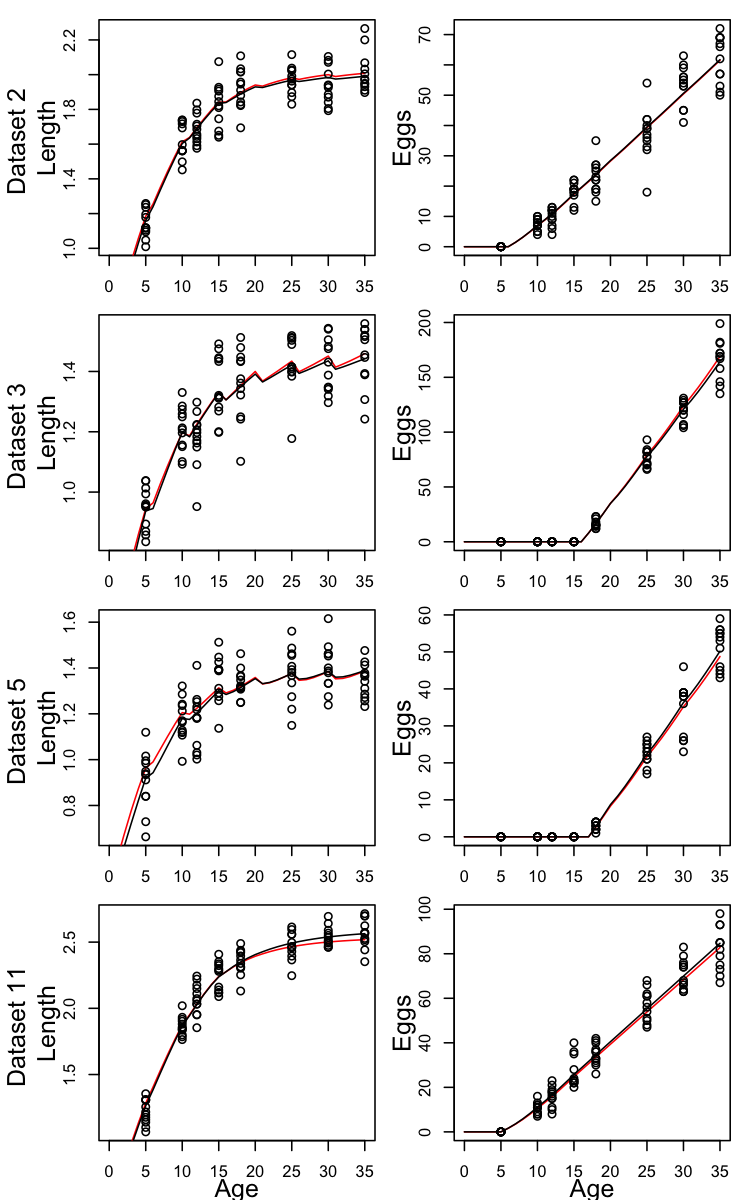
\includegraphics[width=\linewidth]{figure/unnamed-chunk-1-1} \hfill{}



\end{knitrout}

The table shows the results of the fitting of the different models.
You can see that \textbf{the best-supported model has a stage-structured parasite exploiting somatic tissue with a carrying capacity determined by host mass}.
The parameter values are probably not worth taking very seriously, but they are interesting in what they indicate.
In particular, the best-fitting somatic maintenance rate $k_m$ is essentially zero.
This is actually not that surprising, given what we saw earlier, that it is very difficult to fit the growth trajectory.
The other thing to notice is that the negative binomial measurement error estimates $P_{err}$ are always very small, which greatly inflates the variance.
However, the mean trajectories for growth of infected animals and spore production actually look pretty good (Fig. \ref{fig:best-fit}).




\begin{knitrout}\scriptsize
\definecolor{shadecolor}{rgb}{0.969, 0.969, 0.969}\color{fgcolor}\begin{figure}

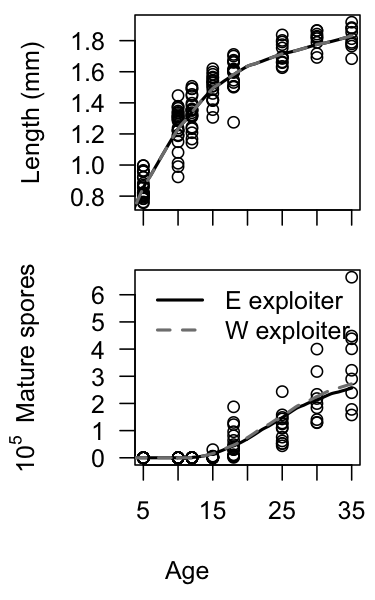
\includegraphics[width=\linewidth]{figure/best-fit-1} \hfill{}

\caption[Infected animal growth and spore production for the two best fitting models]{Infected animal growth and spore production for the two best fitting models. You can see that the models predict essentially identical growth and mature spore production.}\label{fig:best-fit}
\end{figure}


\end{knitrout}

\end{document}
